\section{Working with GTFS data}
\label{sec:gtfs}

GTFS (general transit feed specification)
is an API (application programming interface) specification for transit data,
developed and maintained by Google \citep{GoogleDevelopers_2006}.
It is used by over 900~transit providers around the world,
including here in Auckland, New Zealand
(source \url{http://transitfeeds.com}),
allowing an application developed in Auckland to
be deployed to another GTFS-based public transport system with minimal modification.


The two main components of GTFS are \emph{static} and \emph{realtime}.
Static GTFS includes information about routes, trips, shapes, and stops:
a \emph{route} is a sequence of two or more stops displayed as a single service;
a \emph{trip} is an instance of a route occuring at a specific time of day;
a \emph{shape} is the sequence of points defining a vehicle's path along a route;
and a \emph{stop} is a physical location where passengers can embark and disembark
the vehicle \citep{GoogleDevelopers_2006}.
GTFS realtime feeds provide information such as vehicle positions and trip delays,
and are usually accessed via an API.
% The latter is often the only covariate used for predicting arrival time,
% as previously discussed:
% while it is a computationally inexpensive method (simply addition),
% it relies on accurate schedules and cannot respond quickly to realtime events.

\subsection{Transit network construction}
\label{sec:network_build}

Arguably one of the most important predictors of arrival time is
the travel time along intermediate roads,
however in most applications this vital information is unavailable,
at least directly. 
Several predictive approaches used \emph{headway},
the time between consecutive trips along the same route
\citep{Hans_2015}.
While this is reasonable for high frequency routes,
low frequncy routes will be unable to react quickly to changes in congestion,
and it is for these routes which reliable ETAs are arguably more important,
since the cost of missing a bus is greater.


One solution would be to use information obtained from
vehicles servicing other routes but traveling along the same roads
to estimate arrival times;
however, there is no direct way of knowing which routes share common roads.
Here we propose using an algorithm to convert the raw GTFS shape files
into a \emph{road network},
as demonstated in Figure~\ref{fig:network_creation}.
This involves detecting locations where one or more routes meet 
(intersections or \emph{nodes}),
and the connecting paths (road segments or \emph{edges}).
However, in this paper we use bus stops as nodes and the routes between them as edges.
This captures most overlaps, 
with the exception of some express services and multiple-stop locations,
but these are typically in high traffic areas and should be OK.
Figure~\ref{fig:network_creation_2} demonstrates how several overlapping routes 
are merged to form a road network.
In section~\ref{sec:kf} we present a model for estimating veihcle travel time
along a road segment.

\begin{figure}[tb]
    \centering
    \begin{subfigure}{0.7\textwidth}
        \centering
        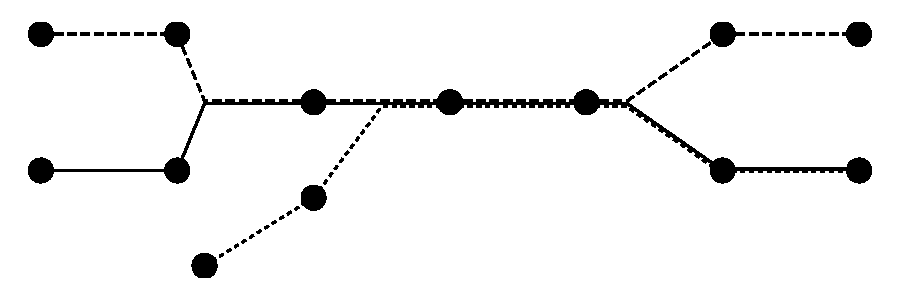
\includegraphics[width=0.95\textwidth]{figures/02_network_segments_1.pdf}
        \caption{Raw GTFS route shapes}
        \label{fig:network_creation_1}
    \end{subfigure} \\
    \begin{subfigure}{0.7\textwidth}
        \centering
        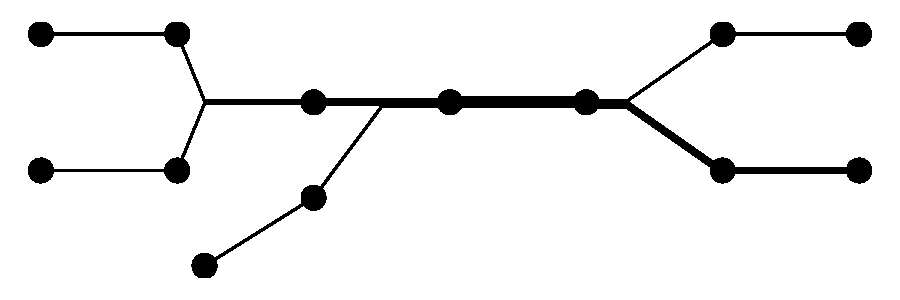
\includegraphics[width=0.95\textwidth]{figures/02_network_segments_2.pdf}
        \caption{GTFS-based road network}
        \label{fig:network_creation_2}
    \end{subfigure}
    \caption{Construction of a route network involves combining routes at nodes %
        (here we are using stops) which are connected by edges (roads). %
        In (a), the three unique routes, represented by different line types, clearly %
        overlap in several places. In (b) these have been merged, and the width of each line %
        represents how many routes use that link.}
    \label{fig:network_creation}
\end{figure}


\subsection{Realtime vehicle locations}
\label{sec:realtime_data}

GTFS \rt allows developers to query the current positions of vehicles
in the transit network.
The data consists of the time $t_k$ that the observation was made,
the GPS position of the vehicle, $\bY_k$, 
and some other information about the trip being serviced.
Vehicle positions are updated with a frequency of anywhere from 10~seconds to several minutes,
so there is often a lot of uncertainty about the trajectory
between two observations, particularly when there is a bus stop
or intersection between them.

Another complication with the Auckland Transport realtime feed is that
the buses are programmed to report their location when arriving at
bus stops and some major intersections.
Often these positions appear to be preemptive (i.e., that bus is almost there, 
but not quite),
and subsequent observations place the bus \emph{behind} the stop or intersection.
To handle this, we compute the approximate distance traveled, $\tilde x_k$,
of the vehicle by finding the nearest point on the path to the observation;
if this has decreased, the previous observation is rejected and the vehicle reverted
to its previous state.
To enable this, vehicles retain the current and previous states (see section~\ref{sec:rt}).
